\section{接收端窗口值}
\subsection{简述接收端窗口值}
在TCP协议中影响数据发送的三个因素分别为:发送端窗口值、接收端窗口值和拥塞窗口值。本文主要分析MPTCP中各个子路径对接收端窗口值rcv\_wnd的处理。
\subsection{接收端窗口值的初始化}
根据《MPTCP 源码分析(二) 建立子路径》中描述服务端在发送完SYN/ACK并接收到ACK的时候建立新的sock。在内核实现中,针对连接请求分为两个步骤处理:
\begin{itemize}
  \item SYN队列处理:当服务端收到SYN的时候,此连接请求request\_sock将被存放于listening socket的SYN队列,服务端发送SYN/ACK并等待相应的ACK。
  \item accept队列处理:一旦等待的ACK收到,服务端将会创建新的socket,并将连接请求从listening socket的SYN队列移到其accept队列。
\end{itemize}
当服务端进入LINSTEN状态后,收到第一个SYN包后的处理流程如下:
\begin{figure}[H]
  \centering
  % Requires \usepackage{graphicx}
  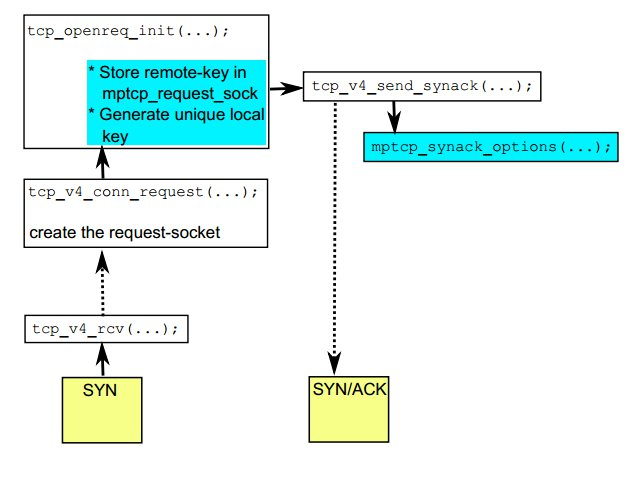
\includegraphics[width=10cm]{dias/Handle-first-SYN.jpg}\\
  \caption{处理第一个SYN包}
\end{figure}
详细的函数调用为:
\small\begin{verbatim}
tcp_v4_rcv
               =》 tcp_v4_do_rcv
                     =》 tcp_rcv_state_process
                         =》mptcp_conn_request
                              =》tcp_v4_conn_request
                                   =》tcp_conn_request
                                        =》tcp_openreq_init
\end{verbatim}\normalsize
在函数tcp\_conn\_request中对连接请求request\_sock进行了分配内存。
\small\begin{verbatim}
"net/ipv4/tcp_input.c" line 6097 of 6195
6097     req = inet_reqsk_alloc(rsk_ops);
6098     if (!req)
6099         goto drop;
\end{verbatim}\normalsize
在函数tcp\_openreq\_init中对request\_sock进行了初始化操作。
\small\begin{verbatim}
1226 static inline void tcp_openreq_init(struct request_sock *req,
1227                     struct tcp_options_received *rx_opt,
1228                     struct sk_buff *skb)
1229 {
1230     struct inet_request_sock *ireq = inet_rsk(req);
1231
1232     req->rcv_wnd = 0;       /* So that tcp_send_synack() knows! */
1233     req->cookie_ts = 0;
1234     tcp_rsk(req)->rcv_isn = TCP_SKB_CB(skb)->seq;
1235     tcp_rsk(req)->rcv_nxt = TCP_SKB_CB(skb)->seq + 1;
1236     tcp_rsk(req)->snt_synack = 0;
1237     req->mss = rx_opt->mss_clamp;
1238     req->ts_recent = rx_opt->saw_tstamp ? rx_opt->rcv_tsval : 0;
1239     ireq->tstamp_ok = rx_opt->tstamp_ok;
1240     ireq->sack_ok = rx_opt->sack_ok;
1241     ireq->snd_wscale = rx_opt->snd_wscale;
1242     ireq->wscale_ok = rx_opt->wscale_ok;
1243     ireq->acked = 0;
1244     ireq->ecn_ok = 0;
1245     ireq->mptcp_rqsk = 0;
1246     ireq->saw_mpc = 0;
1247     ireq->ir_rmt_port = tcp_hdr(skb)->source;
1248     ireq->ir_num = ntohs(tcp_hdr(skb)->dest);
1249 }
\end{verbatim}\normalsize
第1232行对request\_sock的rcv\_wnd进行了初始化为0。

当服务端收到ACK的时候就会建立相应的socket。将会调用tcp\_create\_openreq\_child函数实现,定义如下:
\small\begin{verbatim}
    "include/net/tcp.h" line 578 of 1787
    struct sock *tcp_create_openreq_child(struct sock *sk,
                          struct request_sock *req,
                          struct sk_buff *skb);
\end{verbatim}\normalsize
对于rcv\_wnd的处理具体如下:
\small\begin{verbatim}
"net/ipv4/tcp_minisocks.c" line 441 of 872
512         newtp->window_clamp = req->window_clamp;
513         newtp->rcv_ssthresh = req->rcv_wnd;
514         newtp->rcv_wnd = req->rcv_wnd;
515         newtp->rx_opt.wscale_ok = ireq->wscale_ok;
\end{verbatim}\normalsize
这个阶段为MPTCP的第一条子路径建立情况的三次握手,因此此时创建的socket的属性为master而非slave.

下面的情景为创建一条子路径的情况,当服务端收到第一个SYN包的函数调用情况如下:
\begin{figure}
  \centering
  % Requires \usepackage{graphicx}
  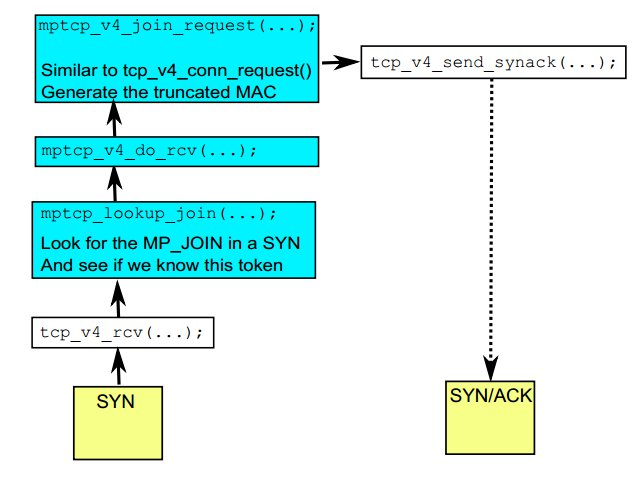
\includegraphics[width=10cm]{dias/Receive-first-SYN.jpg}\\
  \caption{服务端收到第一个SYN包}
\end{figure}
函数mptcp\_v4\_join\_request将会对连接请求request\_sock进行内存分配并初始化。具体的调用如下:
\small\begin{verbatim}
    mptcp_v4_join_request
                           =》tcp_conn_request
                                =》inet_reqsk_alloc
                                =》tcp_openreq_init
\end{verbatim}\normalsize
当客户端的ACK到达后,内核会将此连接请求request\_sock的rcv\_wnd赋值给slave subsocket.
\subsection{master sock 和 slave sock之间接收端窗口值的关系}
TCP在发包的时候会告诉对方自身的接收端窗口值。MPTCP的实现如下:
\small\begin{verbatim}
"net/mptcp/mptcp_output.c" line 992 of 1667
992 u16 mptcp_select_window(struct sock *sk)
993 {
994     u16 new_win     = tcp_select_window(sk);
995     struct tcp_sock *tp = tcp_sk(sk);
996     struct tcp_sock *meta_tp = mptcp_meta_tp(tp);
997
998     meta_tp->rcv_wnd    = tp->rcv_wnd;
999     meta_tp->rcv_wup    = meta_tp->rcv_nxt;
1000
1001     return new_win;
1002 }
\end{verbatim}\normalsize
第994获得最新的窗口值并返回。第998行将slave sock的rcv\_wnd赋值给master sock。

第994行的函数tcp\_select\_window的实现如下:
\small\begin{verbatim}
"net/ipv4/tcp_output.c" line 275 of 3327
275 u16 tcp_select_window(struct sock *sk)
276 {
277     struct tcp_sock *tp = tcp_sk(sk);
278     /* The window must never shrink at the meta-level. At the subflow we
279      * have to allow this. Otherwise we may announce a window too large
280      * for the current meta-level sk_rcvbuf.
281      */
282     u32 cur_win = tcp_receive_window(mptcp(tp) ? tcp_sk(mptcp_meta_sk(sk)) : tp);
283     u32 new_win = tp->__select_window(sk);
\end{verbatim}\normalsize
对于第283行的\_\_select\_window()函数,MPTCP的内核实现如下:
\small\begin{verbatim}
"net/mptcp/mptcp_output.c" line 771 of 1667
771 u32 __mptcp_select_window(struct sock *sk)
772 {
773     struct inet_connection_sock *icsk = inet_csk(sk);
774     struct tcp_sock *tp = tcp_sk(sk), *meta_tp = mptcp_meta_tp(tp);
775     struct sock *meta_sk = mptcp_meta_sk(sk);
776     int mss, free_space, full_space, window;
777
778     /* MSS for the peer's data.  Previous versions used mss_clamp
779      * here.  I don't know if the value based on our guesses
780      * of peer's MSS is better for the performance.  It's more correct
781      * but may be worse for the performance because of rcv_mss
782      * fluctuations.  --SAW  1998/11/1
783      */
784     mss = icsk->icsk_ack.rcv_mss;
785     free_space = tcp_space(meta_sk);
786     full_space = min_t(int, meta_tp->window_clamp,
787             tcp_full_space(meta_sk));
788
789     if (mss > full_space)
790         mss = full_space;
791
792     if (free_space < (full_space >> 1)) {
793         icsk->icsk_ack.quick = 0;
794
795         if (tcp_memory_pressure)
796             /* TODO this has to be adapted when we support different
797              * MSS's among the subflows.
798              */
799             meta_tp->rcv_ssthresh = min(meta_tp->rcv_ssthresh,
800                             4U * meta_tp->advmss);
801
802         if (free_space < mss)
803             return 0;
804     }
805
806     if (free_space > meta_tp->rcv_ssthresh)
807         free_space = meta_tp->rcv_ssthresh;
808
809     /* Don't do rounding if we are using window scaling, since the
810      * scaled window will not line up with the MSS boundary anyway.
811      */
812     window = meta_tp->rcv_wnd;
813     if (tp->rx_opt.rcv_wscale) {
814         window = free_space;
815
816         /* Advertise enough space so that it won't get scaled away.
817          * Import case: prevent zero window announcement if
818          * 1<<rcv_wscale > mss.
819          */
820         if (((window >> tp->rx_opt.rcv_wscale) << tp->
821              rx_opt.rcv_wscale) != window)
822             window = (((window >> tp->rx_opt.rcv_wscale) + 1)
823                   << tp->rx_opt.rcv_wscale);
824     } else {
825         /* Get the largest window that is a nice multiple of mss.
826          * Window clamp already applied above.
827          * If our current window offering is within 1 mss of the
828          * free space we just keep it. This prevents the divide
829          * and multiply from happening most of the time.
830          * We also don't do any window rounding when the free space
831          * is too small.
832          */
833         if (window <= free_space - mss || window > free_space)
834             window = (free_space / mss) * mss;
835         else if (mss == full_space &&
836              free_space > window + (full_space >> 1))
837             window = free_space;
838     }
839
840     return window;
841 }
\end{verbatim}\normalsize
影响window的计算的因素为:
\begin{itemize}
  \item 收到的MSS( icsk$\rightarrow$icsk\_ack.rcv\_mss)
  \item 套接字缓冲区总的空间(tcp\_full\_space)
  \item 套接字缓冲区的空闲空间(tcp\_space)
  \item meta\_tp$\rightarrow$rcv\_ssthresh  /* Current window clamp */
\end{itemize}
观察上面的代码可以知道MPTCP的实现和\_\_tcp\_select\_window的区别是都是依据meta\_tp,而非tp。这说明master sock 和 其余slave sock使用相同的 rcv\_wnd。
\subsection{结论}
\begin{itemize}
  \item master sock 和 其余slave sock使用相同的接收缓冲区和 rcv\_wnd。
\end{itemize}